\documentclass[a4paper,11pt]{article}

\usepackage[italian]{babel}

\usepackage[latin1]{inputenc}

\usepackage[T1]{fontenc}

\usepackage{graphicx}

\usepackage{indentfirst}

\usepackage{amsmath,amssymb}

\usepackage{enumitem} 

\newcommand{\virgolette}[1]{``#1''}

\usepackage[margin=1in]{geometry} %Smaller margins

\usepackage{lmodern} %Vector PDF

\usepackage{siunitx}

\usepackage{xcolor}

\usepackage{colortbl}

\usepackage{multirow}

\usepackage{rotating}

\usepackage{booktabs}

\usepackage{longtable}

\usepackage{graphicx}
\graphicspath{ {Images/} }

\usepackage{wrapfig}

\newcommand*\chem[1]{\ensuremath{\mathrm{#1}}}

\begin{document}

		\section{Presentazione ed analisi dei dati}
		
		L'analisi dei dati di questo esperimento pu� essere separata in due sezioni. Da una parte infatti � possibile estrarre, dai dati ricavati in laboratorio, gli indici di rifrazione $n_\lambda$ del prisma relativi alle lunghezze d'onda dello spettro di emissione del mercurio. In secondo luogo invece � possibile osservare e verificare che la relazione \ref{Cauchy} intercorre tra i dati acquisiti.
		
%		\begin{equation}\label{retta}
%		 n_{\lambda}^{2} = \frac{m}{\lambda^2} + q; \;\; m,q \in \mathbb{R}.
%		\end{equation}
		
		
		
		\subsection{Presentazione dei Dati}
		
		Per quanto riguarda la presentazione dei dati raccolti occorre fare alcune precisazioni. In primo luogo come lunghezze d'onda sono state utilizzate quelle ricavate sperimentalmente nella sessione di laboratorio precedente. Tra queste poi non sono state considerate quelle particolari $\lambda$ che, nonostante in teoria dovessero essere visibili, non sono state osservate durante la sessione di laboratorio. In sostanza le $\lambda$ di riferimento sono le seguenti\footnote{La nomenclatura utilizzata fa riferimento alla relazione precedente.}:
		
		\begin{table}[htbp]
			\centering
			\caption{Lunghezze d'onda dello spettro di emissione del Mercurio attraverso il prisma}
			\medskip
			\begin{tabular}{lrr}
				\bottomrule
				\rowcolor[rgb]{ .267,  .447,  .769} \textcolor[rgb]{ 1,  1,  1}{\textbf{Colore}} & \multicolumn{1}{l}{\textcolor[rgb]{ 1,  1,  1}{\textbf{$\lambda$ (nm)}}} & \multicolumn{1}{l}{\textcolor[rgb]{ 1,  1,  1}{\textbf{$\sigma _\lambda$ (nm)}}} \\
				\toprule
				\rowcolor[rgb]{ .267,  .447,  .769} \textcolor[rgb]{ 1,  1,  1}{\textbf{Viola interno}} & \cellcolor[rgb]{ .851,  .851,  .851} 404.632 & \cellcolor[rgb]{ .851,  .851,  .851} 0.395 \\
				\rowcolor[rgb]{ .267,  .447,  .769} \textcolor[rgb]{ 1,  1,  1}{\textbf{Viola esterno}} & \cellcolor[rgb]{ 1,  1,  1} 407.802 & \cellcolor[rgb]{ 1,  1,  1} 0.515 \\
				\rowcolor[rgb]{ .267,  .447,  .769} \textcolor[rgb]{ 1,  1,  1}{\textbf{Blu}} & \cellcolor[rgb]{ .851,  .851,  .851} 435.829 & \cellcolor[rgb]{ .851,  .851,  .851} 0.301\\
				\rowcolor[rgb]{ .267,  .447,  .769} \textcolor[rgb]{ 1,  1,  1}{\textbf{Verde interno}} & \cellcolor[rgb]{ 1,  1,  1} 492.283 & \cellcolor[rgb]{ 1,  1,  1} 0.501 \\
				\rowcolor[rgb]{ .267,  .447,  .769} \textcolor[rgb]{ 1,  1,  1}{\textbf{Verde giallo}} & \cellcolor[rgb]{ .851,  .851,  .851} 546.037 & \cellcolor[rgb]{ .851,  .851,  .851} 0.274\\
				\rowcolor[rgb]{ .267,  .447,  .769} \textcolor[rgb]{ 1,  1,  1}{\textbf{Giallo interno}} & \cellcolor[rgb]{ 1,  1,  1} 576.942 & \cellcolor[rgb]{ 1,  1,  1} 0.300 \\
				\rowcolor[rgb]{ .267,  .447,  .769} \textcolor[rgb]{ 1,  1,  1}{\textbf{Giallo esterno}} &\cellcolor[rgb]{ .851,  .851,  .851} 579.006 & \cellcolor[rgb]{ .851,  .851,  .851} 0.299 \\
				
				\toprule
			\end{tabular}%
			\label{lambda}%
		\end{table}%
		
		Per il calcolo dell'angolo $\alpha$, come da procedura indicata nella sezione precedente, sono state ripetute pi� misure indipendenti. I valori sono riportati nella tabella \ref{alpha}.
		
		\begin{table}[htbp]
			\centering
			\caption{Dati per la determinazione del valore dell'angolo $\alpha$.}
			\medskip
			\begin{tabular}{lrrrrrr}
				\bottomrule
				\rowcolor[rgb]{ .267,  .447,  .769} \textcolor[rgb]{ 1,  1,  1}{\textbf{No misura}} & \multicolumn{1}{l}{\textcolor[rgb]{ 1,  1,  1}{\textbf{$\theta_1$}(rad)}} & \multicolumn{1}{l}{\textcolor[rgb]{ 1,  1,  1}{\textbf{$\sigma _{\theta_1}$(rad)}}} & \multicolumn{1}{l}{\textcolor[rgb]{ 1,  1,  1}{\textbf{$\theta_2$(rad)}}} & \multicolumn{1}{l}{\textcolor[rgb]{ 1,  1,  1}{\textbf{$\sigma _{\theta_2}$(rad)}}} & \multicolumn{1}{l}{\textcolor[rgb]{ 1,  1,  1}{\textbf{$\alpha$(rad)}}} & \multicolumn{1}{l}{\textcolor[rgb]{ 1,  1,  1}{\textbf{$\sigma _\alpha$(rad)}}}\\
				\toprule
				\rowcolor[rgb]{ .267,  .447,  .769} \textcolor[rgb]{ 1,  1,  1}{\textbf{1}} & \cellcolor[rgb]{ .851,  .851,  .851} 6.186029 & \cellcolor[rgb]{ .851,  .851,  .851} 0.000292 & \cellcolor[rgb]{ .851,  .851,  .851} 0.949459 & \cellcolor[rgb]{ .851,  .851,  .851} 0.000292 & \cellcolor[rgb]{ .851,  .851,  .851} 1.046615 & \cellcolor[rgb]{ .851,  .851,  .851} 0.000583 \\
				
				\rowcolor[rgb]{ .267,  .447,  .769} \textcolor[rgb]{ 1,  1,  1}{\textbf{2}} & \cellcolor[rgb]{ 1,  1,  1} 0.624261 & \cellcolor[rgb]{ 1,  1,  1} 0.000292 & \cellcolor[rgb]{ 1,  1,  1} 4.812164 & \cellcolor[rgb]{ 1,  1,  1} 0.000292 & \cellcolor[rgb]{ 1,  1,  1} 1.046325 & \cellcolor[rgb]{ 1,  1,  1} 0.000583 \\
				\rowcolor[rgb]{ .267,  .447,  .769} \textcolor[rgb]{ 1,  1,  1}{\textbf{3}} & \cellcolor[rgb]{ .851,  .851,  .851} 0.529998 & \cellcolor[rgb]{ .851,  .851,  .851} 0.000292 & \cellcolor[rgb]{ .851,  .851,  .851} 4.717480 & \cellcolor[rgb]{ .851,  .851,  .851} 0.000292 & \cellcolor[rgb]{ .851,  .851,  .851} 1.045889 & \cellcolor[rgb]{ .851,  .851,  .851} 0.000583\\
				\rowcolor[rgb]{ .267,  .447,  .769} \textcolor[rgb]{ 1,  1,  1}{\textbf{4}} & \cellcolor[rgb]{ 1,  1,  1} 0.450295 & \cellcolor[rgb]{ 1,  1,  1} 0.000292 & \cellcolor[rgb]{ 1,  1,  1} 4.638212 & \cellcolor[rgb]{ 1,  1,  1} 0.000292 & \cellcolor[rgb]{ 1,  1,  1} 1.046325 & \cellcolor[rgb]{ 1,  1,  1} 0.000583 \\
				\rowcolor[rgb]{ .267,  .447,  .769} \textcolor[rgb]{ 1,  1,  1}{\textbf{5}} & \cellcolor[rgb]{ .851,  .851,  .851} 0.448259 & \cellcolor[rgb]{ .851,  .851,  .851} 0.000292 & \cellcolor[rgb]{ .851,  .851,  .851} 4.636176 & \cellcolor[rgb]{ .851,  .851,  .851} 0.000292 & \cellcolor[rgb]{ .851,  .851,  .851} 1.046325 & \cellcolor[rgb]{ .851,  .851,  .851} 0.000583 \\
				\rowcolor[rgb]{ .267,  .447,  .769} \textcolor[rgb]{ 1,  1,  1}{\textbf{6}} & \cellcolor[rgb]{ 1,  1,  1} 0.535089 & \cellcolor[rgb]{ 1,  1,  1} 0.000292 & \cellcolor[rgb]{ 1,  1,  1} 4.723443 & \cellcolor[rgb]{ 1,  1,  1} 0.000292 & \cellcolor[rgb]{ 1,  1,  1} 1.046761 & \cellcolor[rgb]{ 1,  1,  1} 0.000583\\				
				\toprule
			\end{tabular}%
			\label{alpha}%
		\end{table}%
		
		Elaborando statisticamente i dati, tramite calcolo della media e di deviazione standard\footnote{Il controllo sulla compatibilit� dei valori ottenuti � evidente e giustifica l'utilizzo di media e deviazione.}, si ottiene un valore finale
		\[\alpha = 1.046373 \pm 0.000300 \; \si{rad} .\]
		
		La determinazione degli angoli di deviazione minima per le lunghezze d'onda � stata effettuata con una analoga procedura di ripetizione delle misure. In questo caso, noto l'angolo $\delta_0 = 3.126958 \pm 0.000292 \; \si{rad}$, il valore di $\delta_m(\lambda)$ si ottiene per differenza. Le misure effettuate e riportate nella tabella \ref{delta} fanno riferimento a un numero eguale di misurazioni compiute in senso orario e anti-orario rispetto all'angolo $\delta_0$:\footnote{Le misure riportate si riferiscono ai valori calcolati di $\delta_m(\lambda)$ tramite analisi statistica con media e deviazione. In appendice vengono riportate le misure originali da cui questi dati sono stati estratti.}
		
		\begin{table}[htbp]
			\centering
			\caption{Angoli di deviazione minima.}
			\medskip
			\begin{tabular}{lrr}
				\bottomrule
				\rowcolor[rgb]{ .267,  .447,  .769} \textcolor[rgb]{ 1,  1,  1}{\textbf{Colore}} & \multicolumn{1}{l}{\textcolor[rgb]{ 1,  1,  1}{\textbf{$\delta$ (rad)}}} & \multicolumn{1}{l}{\textcolor[rgb]{ 1,  1,  1}{\textbf{$\sigma _\delta$ (rad)}}} \\
				\toprule
				\rowcolor[rgb]{ .267,  .447,  .769} \textcolor[rgb]{ 1,  1,  1}{\textbf{Viola interno}} & \cellcolor[rgb]{ .851,  .851,  .851} 1.298476 & \cellcolor[rgb]{ .851,  .851,  .851} 0.000583 \\
				\rowcolor[rgb]{ .267,  .447,  .769} \textcolor[rgb]{ 1,  1,  1}{\textbf{Viola esterno}} & \cellcolor[rgb]{ 1,  1,  1} 1.293153 & \cellcolor[rgb]{ 1,  1,  1} 0.000583 \\
				\rowcolor[rgb]{ .267,  .447,  .769} \textcolor[rgb]{ 1,  1,  1}{\textbf{Blu}} & \cellcolor[rgb]{ .851,  .851,  .851} 1.255771 & \cellcolor[rgb]{ .851,  .851,  .851} 0.000583\\
				\rowcolor[rgb]{ .267,  .447,  .769} \textcolor[rgb]{ 1,  1,  1}{\textbf{Verde interno}} & \cellcolor[rgb]{ 1,  1,  1} 1.207208 & \cellcolor[rgb]{ 1,  1,  1} 0.000583 \\
				\rowcolor[rgb]{ .267,  .447,  .769} \textcolor[rgb]{ 1,  1,  1}{\textbf{Verde giallo}} & \cellcolor[rgb]{ .851,  .851,  .851} 1.177580 & \cellcolor[rgb]{ .851,  .851,  .851} 0.000583\\
				\rowcolor[rgb]{ .267,  .447,  .769} \textcolor[rgb]{ 1,  1,  1}{\textbf{Giallo interno}} & \cellcolor[rgb]{ 1,  1,  1} 1.165038 & \cellcolor[rgb]{ 1,  1,  1} 0.000583 \\
				\rowcolor[rgb]{ .267,  .447,  .769} \textcolor[rgb]{ 1,  1,  1}{\textbf{Giallo esterno}} &\cellcolor[rgb]{ .851,  .851,  .851} 1.163969 & \cellcolor[rgb]{ .851,  .851,  .851} 0.000583 \\
				
				\toprule
			\end{tabular}%
			\label{delta}%
		\end{table}%
	
		\subsection{Elaborazione dei dati e presentazione dei risultati - Indici di Rifrazione}
		
		I dati riportati nella sezione precedente sono sufficienti per poter ricavare dei valori relativi all'indice di rifrazione $n$ del materiale di cui � composto il prisma come funzione della lunghezza d'onda $\lambda$ della luce incidente. Riportiamo per comodit� la formula da cui si ricava il valore di $n_\lambda$ (l'equazione \ref{n} in introduzione):
		
		\[ n_\lambda = \frac{\sin\frac{\alpha+\delta_\lambda}{2}}{\sin\frac{\alpha}{2}}\]

		dove $\delta_\lambda$ rappresenta il valore dell'angolo di deviazione minima associato a una particolare lunghezza d'onda, riportato anche nella tabella \ref{delta}. Per quanto concerne invece l'errore su $n_\lambda$, questo si ottiene dalle formule di propagazione, derivando rispettivamente rispetto sia a $\lambda$ che ad $\alpha$:
		
		\[ \sigma_n = \sqrt{\left(\frac{\partial n}{\partial \delta} \sigma_\lambda \right)^2 + \left(\frac{\partial n}{\partial \alpha} \sigma_\alpha \right)^2}\]
		ove le derivate parziali sono rispettivamente
		\[ \frac{\partial n}{\partial \delta} = \frac{\cos\frac{\alpha+\delta_\lambda}{2}}{\sin\frac{\alpha}{2}} \]
		e
		\[\frac{\partial n}{\partial \alpha} = \frac{\sin\frac{- \delta_\lambda}{2}}{2\left(\sin\frac{\alpha}{2}\right)^2} \; \; .\]
		
		I valori ottenuti per $n$ relativamente ad ognuna delle lunghezze d'onda considerate sono riportati nella tabella \ref{indici}.
		
		\begin{table}[htbp]
			\centering
			\caption{Valori degli indici di rifrazione in funzione della lunghezza d'onda.}
			\medskip
			\begin{tabular}{lrr}
				\bottomrule
				\rowcolor[rgb]{ .267,  .447,  .769} \textcolor[rgb]{ 1,  1,  1}{\textbf{Colore}} & \multicolumn{1}{l}{\textcolor[rgb]{ 1,  1,  1}{\textbf{$n$ (-)}}} & \multicolumn{1}{l}{\textcolor[rgb]{ 1,  1,  1}{\textbf{$\sigma n$ (-)}}} \\
				\toprule
				\rowcolor[rgb]{ .267,  .447,  .769} \textcolor[rgb]{ 1,  1,  1}{\textbf{Viola interno}} & \cellcolor[rgb]{ .851,  .851,  .851} 1.844704 & \cellcolor[rgb]{ .851,  .851,  .851} 0.000742 \\
				\rowcolor[rgb]{ .267,  .447,  .769} \textcolor[rgb]{ 1,  1,  1}{\textbf{Viola esterno}} & \cellcolor[rgb]{ 1,  1,  1} 1.842632 & \cellcolor[rgb]{ 1,  1,  1} 0.000740 \\
				\rowcolor[rgb]{ .267,  .447,  .769} \textcolor[rgb]{ 1,  1,  1}{\textbf{Blu}} & \cellcolor[rgb]{ .851,  .851,  .851}  1.827707  & \cellcolor[rgb]{ .851,  .851,  .851} 0.000726\\
				\rowcolor[rgb]{ .267,  .447,  .769} \textcolor[rgb]{ 1,  1,  1}{\textbf{Verde interno}} & \cellcolor[rgb]{ 1,  1,  1} 1.807367 & \cellcolor[rgb]{ 1,  1,  1} 0.000709 \\
				\rowcolor[rgb]{ .267,  .447,  .769} \textcolor[rgb]{ 1,  1,  1}{\textbf{Verde giallo}} & \cellcolor[rgb]{ .851,  .851,  .851} 1.794433 & \cellcolor[rgb]{ .851,  .851,  .851} 0.000698\\
				\rowcolor[rgb]{ .267,  .447,  .769} \textcolor[rgb]{ 1,  1,  1}{\textbf{Giallo interno}} & \cellcolor[rgb]{ 1,  1,  1} 1.788839 & \cellcolor[rgb]{ 1,  1,  1} 0.000694 \\
				\rowcolor[rgb]{ .267,  .447,  .769} \textcolor[rgb]{ 1,  1,  1}{\textbf{Giallo esterno}} &\cellcolor[rgb]{ .851,  .851,  .851} 1.788359 & \cellcolor[rgb]{ .851,  .851,  .851} 0.000694 \\
				
				\toprule
			\end{tabular}%
			\label{indici}%
		\end{table}%
		
		
		\subsection{Elaborazione dei dati e presentazione dei risultati - Regressione Lineare}
		Chiaramente di per s� questi valori sono poco indicativi, nella misura in cui non si hanno termini di confronto con cui testarne la compatibilit�. Tuttavia l'equazione \ref{Cauchy} suggerisce che la bont� delle misure effettuate -- a meno di errori sistematici -- possa essere testata proprio trovando la miglior retta passante per i punti del piano $(n_{\lambda}^{2}, \frac{1}{\lambda ^2})$.

		\begin{wrapfigure}{l}{0.5\textwidth}
			\caption{Grafico della regressione}\label{regr}
				\centering
				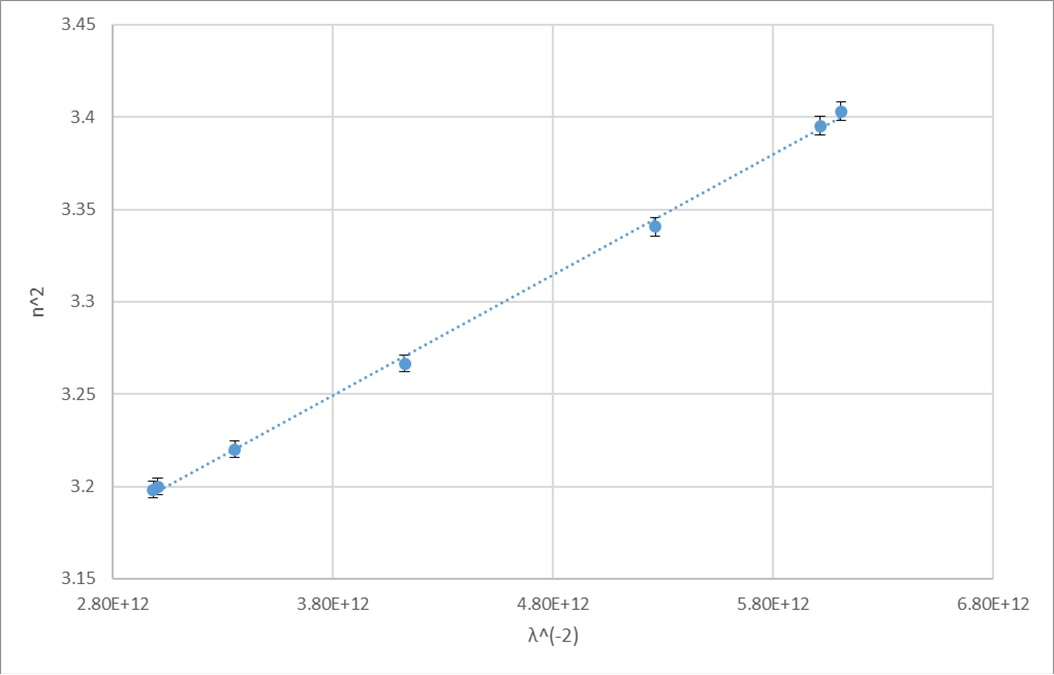
\includegraphics[width=0.5\textwidth]{Retta}
		\end{wrapfigure}

		
		In merito all'utilizzo dell'algoritmo di regressione lineare occorre tuttavia una precisazione. I dati che abbiamo a disposizione sia per quanto riguarda l'asse delle $x$ che quello delle $y$ hanno errore variabile. In una situazione del genere non � teoricamente possibile utilizzare l'algoritmo di regressione nella forma pesata. Quello che si osserva � per� che se si calcola il coefficiente angolare della retta trascurando gli errori, e si sommano in quadratura gli errori di ascisse e ordinate, il risultato differisce alla quarta cifra significativa rispetto a $\sigma_{n^2}$. Il contributo dell'errore su $\frac{1}{\lambda ^2}$ � dunque $10^{-4}$ volte significativo rispetto a quello di $n^2$. In considerazione di questo fatto abbiamo adottato l'algoritmo di regressione pesata\footnote{\'E evidente che la procedura adottata non pu� essere considerata formalmente inattaccabile, in quanto per scegliere quale tipo di algoritmo di regressione lineare abbiamo calcolato uno dei termini incogniti dell'algoritmo di regressione con un metodo meno raffinato. Quello che giustifica la scelta presente � il fatto, osservabile solo a posteriori, che l'errore sulle ordinate ha un contributo nel calcolo dei termini di regressione molto superiore rispetto a quello sulle ascisse.}.
		
		In tabella \ref{regressione} vengono riportati i dati tramite i quali � stato effettuato il calcolo di coefficiente angolare e intercetta per la retta e nella figura \ref{regr} viene riportato il grafico di $ n^2 \text{ e } \lambda^{-2} $ e la relativa retta di regressione.
			
		
		\begin{table}[htbp]
			\centering
			\caption{Dati per la regressione lineare.}
			\medskip
			\begin{tabular}{lrrrr}
				\bottomrule
				\rowcolor[rgb]{ .267,  .447,  .769} \textcolor[rgb]{ 1,  1,  1}{\textbf{Colore}} & \multicolumn{1}{l}{\textcolor[rgb]{ 1,  1,  1}{\textbf{$n^2$ (-)}}} & \multicolumn{1}{l}{\textcolor[rgb]{ 1,  1,  1}{\textbf{$\sigma _{n^2}$ (-)}}} & \multicolumn{1}{l}{\textcolor[rgb]{ 1,  1,  1}{\textbf{$\frac{1}{\lambda ^2}$ ($\frac{1}{nm^2}$)}}} & \multicolumn{1}{l}{\textcolor[rgb]{ 1,  1,  1}{\textbf{$\sigma {\frac{1}{\lambda^2}}$ ($\frac{1}{nm^2}$)}}} \\
				\toprule
				\rowcolor[rgb]{ .267,  .447,  .769} \textcolor[rgb]{ 1,  1,  1}{\textbf{Viola interno}} & \cellcolor[rgb]{ .851,  .851,  .851} 3.402935 & \cellcolor[rgb]{ .851,  .851,  .851} 0.005048 & \cellcolor[rgb]{ .851,  .851,  .851} 6.10779E12 & \cellcolor[rgb]{ .851,  .851,  .851} 0.00119E12 \\
				\rowcolor[rgb]{ .267,  .447,  .769} \textcolor[rgb]{ 1,  1,  1}{\textbf{Viola esterno}} & \cellcolor[rgb]{ 1,  1,  1} 3.395291 & \cellcolor[rgb]{ 1,  1,  1} 0.005024 & \cellcolor[rgb]{ 1,  1,  1} 6.01320E12 & \cellcolor[rgb]{ 1,  1,  1} 0.00089E12 \\
				\rowcolor[rgb]{ .267,  .447,  .769} \textcolor[rgb]{ 1,  1,  1}{\textbf{Blu}} & \cellcolor[rgb]{ .851,  .851,  .851}  3.340514  & \cellcolor[rgb]{ .851,  .851,  .851} 0.004853 & \cellcolor[rgb]{ .851,  .851,  .851} 5.26460E12 & \cellcolor[rgb]{ .851,  .851,  .851} 0.00121E12\\
				\rowcolor[rgb]{ .267,  .447,  .769} \textcolor[rgb]{ 1,  1,  1}{\textbf{Verde interno}} & \cellcolor[rgb]{ 1,  1,  1} 3.266575 & \cellcolor[rgb]{ 1,  1,  1} 0.004632 & \cellcolor[rgb]{ 1,  1,  1} 4.12644E12 & \cellcolor[rgb]{ 1,  1,  1} 0.00084E12 \\
				\rowcolor[rgb]{ .267,  .447,  .769} \textcolor[rgb]{ 1,  1,  1}{\textbf{Verde giallo}} & \cellcolor[rgb]{ .851,  .851,  .851} 3.219989  & \cellcolor[rgb]{ .851,  .851,  .851} 0.004469 & \cellcolor[rgb]{ .851,  .851,  .851} 3.35391E12 & \cellcolor[rgb]{ .851,  .851,  .851} 0.00037E12\\
				\rowcolor[rgb]{ .267,  .447,  .769} \textcolor[rgb]{ 1,  1,  1}{\textbf{Giallo interno}} & \cellcolor[rgb]{ 1,  1,  1} 3.199945 & \cellcolor[rgb]{ 1,  1,  1} 0.004442 & \cellcolor[rgb]{ 1,  1,  1} 3.00427E12 & \cellcolor[rgb]{ 1,  1,  1} 0.00031E12 \\
				\rowcolor[rgb]{ .267,  .447,  .769} \textcolor[rgb]{ 1,  1,  1}{\textbf{Giallo esterno}} &\cellcolor[rgb]{ .851,  .851,  .851} 3.198227 & \cellcolor[rgb]{ .851,  .851,  .851} 0.004437 & \cellcolor[rgb]{ .851,  .851,  .851} 2.98283E12 & \cellcolor[rgb]{ .851,  .851,  .851} 0.00085E12 \\
				
				\toprule
			\end{tabular}%
			\label{regressione}%
		\end{table}%
		
		Per questo set di dati l'algoritmo di regressione pesata restituisce rispettivamente 
		
		\begin{equation}\label{coeff.retta_m}
		m = (6.49762 \;\pm \; 0.14067) \, E-14  
		\end{equation}
		\begin{equation}\label{coeff.retta_q}
		q = 3.00277 \; \pm \; 0.00620
		\end{equation}
		
		Dai valori ricavati � possibile effettuare un test di $\chi^2$ per la verifica della bont� della relazione lineare ricavata dalla regressione. Nel caso particolare dalla formula
		\[
		\chi^2 = \sum_{i=1}^{k+2}\frac{|y_i -mx_i - q|^2}{\sigma_{y_i}^2}
		\]
		
		dove $k$ rappresenta il numero di gradi di libert� del sistema considerato -- in questo caso specifico uguale a 5 -- si ricava un valore di $\chi^2$ pari a $2.605$, associato a un confidence level del 25\% circa, ben al di sotto dunque della soglia critica. 
		
\section{Conclusioni}

%Sono stati riportati i dati e l'analisi di questi relativi all'utilizzo di uno spettrometro con prisma per la determinazione dell'indice di rifrazione di un materiale.
%Si � osservata la dipendenza dell'indice di rifrazione del materiale dalla lunghezza d'onda della luce rifratta e sono stati estratti i valori di questo per le lunghezze d'onda piu significative dello spettro del mercurio. 

I valori ottenuti, che considerati a s� stanti sono poco significativi circa la bont� delle procedure sperimentali adottate, sono stati sottoposti ad analisi statistica per la verifica della legge \ref{Cauchy}. Il fatto che la verifica di questa sia avvenuta con successo � un indice della correttezza delle procedure sperimentali ottenute e dei valori riscontrati.

Non � del tutto possibile escludere errori di natura sistematica in quanto descritto, ma il fatto che le stesse procedure siano state ripetute pi� volte, da soggetti diversi, con risultati simili esclude con buona probabilit� la presenza di \textit{biases} degli sperimentatori nella procedura.
		

\end{document}